\documentclass[tikz,border=8pt]{standalone}
\usepackage{ctex}
\usepackage{amsmath,amssymb,bm}
\usetikzlibrary{arrows.meta,calc,angles,quotes,decorations.pathmorphing,patterns,positioning}
\definecolor{ink}{RGB}{30,43,58}
\definecolor{blue}{RGB}{37,91,166}
\definecolor{orange}{RGB}{219,113,25}
\definecolor{green}{RGB}{39,139,94}
\definecolor{red}{RGB}{192,52,52}
\tikzset{
  line cap=round,line join=round,
  body/.style={draw=ink,very thick},
  axis/.style={-{Latex[length=2.5mm]},draw=ink,very thick},
  vec/.style={-{Latex[length=2.5mm]},draw=blue,very thick},
  force/.style={-{Latex[length=2.5mm]},draw=red,very thick},
  guide/.style={draw=ink!50,dashed},
  dim/.style={{Latex[length=2mm]}-{Latex[length=2mm]},draw=ink!75},
  charge/.style={circle,draw=ink,very thick,fill=white,minimum size=8mm,inner sep=0pt},
  nodept/.style={circle,fill=white,draw=ink,thick,minimum size=4.5mm,inner sep=0pt}
}

\tikzset{mass/.style={circle,draw,fill=white,minimum size=7mm},curve/.style={very thick,blue},rope/.style={very thick,blue},ray/.style={very thick,blue,-{Latex}},impulse/.style={very thick,orange,-{Latex}},resistor/.style={thick,decorate,decoration={zigzag,segment length=3mm,amplitude=1mm}}}
\begin{document}
% 1 question-01
\begin{tikzpicture}[x=1cm,y=1cm]
  \coordinate (O) at (0,0); \coordinate (A) at (-4.8,0); \coordinate (B) at (2.4,0);
  \coordinate (C) at (2.4,-3.2); \coordinate (D) at (2.4,1.6);
  \draw[body,orange] (A)--(B); \draw[body,blue] (C)--(D);
  \fill (O) circle (2.5pt) node[below] {$O$};
  \fill (B) circle (2.5pt) node[below right] {$B$};
  \node[left] at (A) {$A$}; \node[below] at (C) {$C$}; \node[above] at (D) {$D$};
  \draw[dim] (-4.8,.65)--(0,.65) node[midway,above] {$2l_1$};
  \draw[dim] (0,.65)--(2.4,.65) node[midway,above] {$l_1$};
  \draw[dim] (3.1,-3.2)--(3.1,1.6) node[midway,right] {$l_3$};
  \node[right] at (2.55,-1.55) {$BC=\dfrac{2l_3}{3}$};
  \node[right] at (2.55,.72) {$BD=\dfrac{l_3}{3}$};
  \pic[draw=ink,"$\theta$",angle radius=7mm,angle eccentricity=1.25]{angle=O--B--C};
  \node[align=center] at (0,-4.05) {长、短摆臂在 $B$ 点铰接；图示为 $\theta=90^\circ$ 的计算位置};
\end{tikzpicture}

% 2 solution-01
\begin{tikzpicture}[x=1cm,y=1cm]
  \draw[axis] (-5,0)--(5,0) node[right] {$x$}; \draw[axis] (-2,-3.6)--(-2,3.4) node[above] {$y$};
  \coordinate (O) at (-2,0); \coordinate (B) at (1,0); \coordinate (C) at (1,-2.7); \coordinate (D) at (1,1.35);
  \draw[body,orange] (-5,0)--(B); \draw[body,blue] (C)--(D);
  \fill (O) circle (2pt) node[below] {$O$}; \fill (B) circle (2pt) node[below left] {$B$};
  \node[below] at (C) {$C$}; \node[above] at (D) {$D$};
  \draw[vec] (B)--++(0,-1.2) node[right] {$\bm v_B$};
  \draw[vec] (D)--++(1.15,0) node[right] {$\bm v_{D/B}$};
  \draw[vec] (C)--++(-1.55,0) node[left] {$\bm v_{C/B}$};
  \draw[force] (-3.5,0)--++(0,-1.35) node[left] {$\lambda(3l_1)g$};
  \draw[force] (1,-.675)--++(0,-1.35) node[right] {$\lambda l_3g$};
  \node[align=left,anchor=west] at (2.3,2.4)
    {$\bm v_P=\bm v_B+\bm\omega_2\times\bm r_{P/B}$\\[2pt]
     $\bm a_P=\bm a_B-\omega_2^2\bm r_{P/B}$};
  \node[align=center] at (0,-4.25) {速度、加速度均按“铰点平动＋短杆绕铰点转动”合成};
\end{tikzpicture}

% 3 question-02
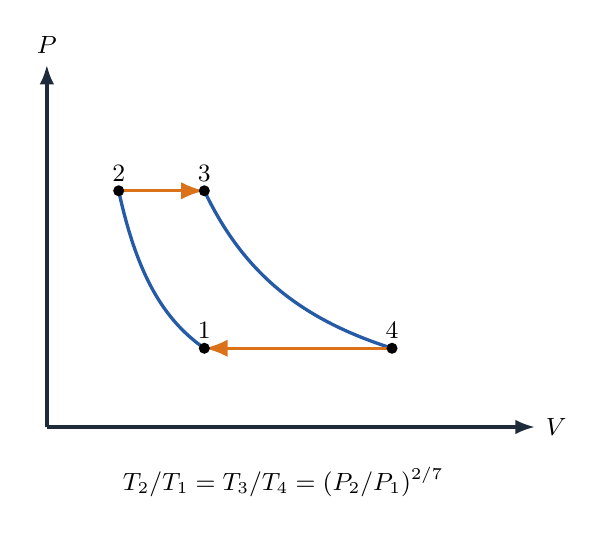
\begin{tikzpicture}[x=1cm,y=1cm,font=\small]
\draw[axis](0,0)--(6.2,0)node[right]{$V$};\draw[axis](0,0)--(0,4.6)node[above]{$P$};\draw[very thick,blue] plot coordinates {(2.000000,1.000000) (1.986234,1.009716) (1.972468,1.019596) (1.958702,1.029642) (1.944936,1.039859) (1.931170,1.050251) (1.917404,1.060823) (1.903639,1.071578) (1.889873,1.082521) (1.876107,1.093658) (1.862341,1.104992) (1.848575,1.116529) (1.834809,1.128275) (1.821043,1.140233) (1.807277,1.152411) (1.793511,1.164813) (1.779745,1.177446) (1.765979,1.190316) (1.752213,1.203428) (1.738447,1.216790) (1.724682,1.230409) (1.710916,1.244291) (1.697150,1.258444) (1.683384,1.272875) (1.669618,1.287591) (1.655852,1.302602) (1.642086,1.317916) (1.628320,1.333541) (1.614554,1.349486) (1.600788,1.365761) (1.587022,1.382375) (1.573256,1.399338) (1.559490,1.416662) (1.545725,1.434356) (1.531959,1.452433) (1.518193,1.470904) (1.504427,1.489781) (1.490661,1.509078) (1.476895,1.528807) (1.463129,1.548982) (1.449363,1.569618) (1.435597,1.590730) (1.421831,1.612333) (1.408065,1.634444) (1.394299,1.657080) (1.380533,1.680259) (1.366768,1.704000) (1.353002,1.728321) (1.339236,1.753243) (1.325470,1.778788) (1.311704,1.804978) (1.297938,1.831836) (1.284172,1.859386) (1.270406,1.887654) (1.256640,1.916667) (1.242874,1.946453) (1.229108,1.977041) (1.215342,2.008463) (1.201576,2.040751) (1.187811,2.073939) (1.174045,2.108063) (1.160279,2.143161) (1.146513,2.179273) (1.132747,2.216440) (1.118981,2.254708) (1.105215,2.294122) (1.091449,2.334732) (1.077683,2.376591) (1.063917,2.419753) (1.050151,2.464276) (1.036385,2.510222) (1.022619,2.557657) (1.008854,2.606649) (0.995088,2.657273) (0.981322,2.709605) (0.967556,2.763730) (0.953790,2.819735) (0.940024,2.877713) (0.926258,2.937766) (0.912492,3.000000)};
\draw[very thick,orange,-{Latex}] plot coordinates {(0.912492,3.000000) (2.000000,3.000000)};
\draw[very thick,blue] plot coordinates {(2.000000,3.000000) (2.030172,2.937766) (2.060344,2.877713) (2.090516,2.819735) (2.120689,2.763730) (2.150861,2.709605) (2.181033,2.657273) (2.211205,2.606649) (2.241377,2.557657) (2.271549,2.510222) (2.301721,2.464276) (2.331894,2.419753) (2.362066,2.376591) (2.392238,2.334732) (2.422410,2.294122) (2.452582,2.254708) (2.482754,2.216440) (2.512927,2.179273) (2.543099,2.143161) (2.573271,2.108063) (2.603443,2.073939) (2.633615,2.040751) (2.663787,2.008463) (2.693959,1.977041) (2.724132,1.946453) (2.754304,1.916667) (2.784476,1.887654) (2.814648,1.859386) (2.844820,1.831836) (2.874992,1.804978) (2.905164,1.778788) (2.935337,1.753243) (2.965509,1.728321) (2.995681,1.704000) (3.025853,1.680259) (3.056025,1.657080) (3.086197,1.634444) (3.116369,1.612333) (3.146542,1.590730) (3.176714,1.569618) (3.206886,1.548982) (3.237058,1.528807) (3.267230,1.509078) (3.297402,1.489781) (3.327575,1.470904) (3.357747,1.452433) (3.387919,1.434356) (3.418091,1.416662) (3.448263,1.399338) (3.478435,1.382375) (3.508607,1.365761) (3.538780,1.349486) (3.568952,1.333541) (3.599124,1.317916) (3.629296,1.302602) (3.659468,1.287591) (3.689640,1.272875) (3.719812,1.258444) (3.749985,1.244291) (3.780157,1.230409) (3.810329,1.216790) (3.840501,1.203428) (3.870673,1.190316) (3.900845,1.177446) (3.931018,1.164813) (3.961190,1.152411) (3.991362,1.140233) (4.021534,1.128275) (4.051706,1.116529) (4.081878,1.104992) (4.112050,1.093658) (4.142223,1.082521) (4.172395,1.071578) (4.202567,1.060823) (4.232739,1.050251) (4.262911,1.039859) (4.293083,1.029642) (4.323255,1.019596) (4.353428,1.009716) (4.383600,1.000000)};
\draw[very thick,orange,-{Latex}] plot coordinates {(4.383600,1.000000) (2.000000,1.000000)};
\fill (2.000000,1.000000) circle(2pt) node[above] {$1$};
\fill (0.912492,3.000000) circle(2pt) node[above] {$2$};
\fill (2.000000,3.000000) circle(2pt) node[above] {$3$};
\fill (4.383600,1.000000) circle(2pt) node[above] {$4$};
\node at(3,-.7){$T_2/T_1=T_3/T_4=(P_2/P_1)^{2/7}$};
\end{tikzpicture}

% 4 solution-02
\begin{tikzpicture}[x=1cm,y=1cm,font=\small]

\draw[axis](0,0)--(5.5,0)node[right]{$S$};\draw[axis](0,0)--(0,4.5)node[above]{$T$};
\draw[very thick,blue,-{Latex}](1,1)--(1,1.369);
\draw[very thick,orange,-{Latex}] plot coordinates {(1.000000,1.368738) (1.037975,1.382402) (1.075949,1.396202) (1.113924,1.410140) (1.151899,1.424217) (1.189873,1.438434) (1.227848,1.452794) (1.265823,1.467297) (1.303797,1.481944) (1.341772,1.496738) (1.379747,1.511679) (1.417722,1.526770) (1.455696,1.542011) (1.493671,1.557405) (1.531646,1.572952) (1.569620,1.588654) (1.607595,1.604513) (1.645570,1.620531) (1.683544,1.636708) (1.721519,1.653047) (1.759494,1.669549) (1.797468,1.686215) (1.835443,1.703048) (1.873418,1.720049) (1.911392,1.737220) (1.949367,1.754562) (1.987342,1.772077) (2.025316,1.789767) (2.063291,1.807634) (2.101266,1.825679) (2.139241,1.843904) (2.177215,1.862312) (2.215190,1.880903) (2.253165,1.899679) (2.291139,1.918643) (2.329114,1.937796) (2.367089,1.957141) (2.405063,1.976678) (2.443038,1.996411) (2.481013,2.016340) (2.518987,2.036469) (2.556962,2.056798) (2.594937,2.077331) (2.632911,2.098068) (2.670886,2.119012) (2.708861,2.140166) (2.746835,2.161531) (2.784810,2.183109) (2.822785,2.204902) (2.860759,2.226913) (2.898734,2.249143) (2.936709,2.271596) (2.974684,2.294272) (3.012658,2.317176) (3.050633,2.340307) (3.088608,2.363670) (3.126582,2.387266) (3.164557,2.411097) (3.202532,2.435166) (3.240506,2.459476) (3.278481,2.484028) (3.316456,2.508825) (3.354430,2.533870) (3.392405,2.559165) (3.430380,2.584712) (3.468354,2.610515) (3.506329,2.636575) (3.544304,2.662895) (3.582278,2.689478) (3.620253,2.716326) (3.658228,2.743442) (3.696203,2.770829) (3.734177,2.798490) (3.772152,2.826426) (3.810127,2.854642) (3.848101,2.883139) (3.886076,2.911920) (3.924051,2.940989) (3.962025,2.970348) (4.000000,3.000000)};
\draw[very thick,blue,-{Latex}](4,3)--(4,2.191);\draw[very thick,orange,-{Latex}] plot coordinates {(4.000000,2.191800) (3.962025,2.170136) (3.924051,2.148686) (3.886076,2.127449) (3.848101,2.106421) (3.810127,2.085601) (3.772152,2.064987) (3.734177,2.044576) (3.696203,2.024368) (3.658228,2.004359) (3.620253,1.984548) (3.582278,1.964932) (3.544304,1.945511) (3.506329,1.926281) (3.468354,1.907242) (3.430380,1.888391) (3.392405,1.869726) (3.354430,1.851245) (3.316456,1.832948) (3.278481,1.814831) (3.240506,1.796893) (3.202532,1.779132) (3.164557,1.761547) (3.126582,1.744136) (3.088608,1.726897) (3.050633,1.709828) (3.012658,1.692928) (2.974684,1.676195) (2.936709,1.659628) (2.898734,1.643224) (2.860759,1.626982) (2.822785,1.610901) (2.784810,1.594979) (2.746835,1.579214) (2.708861,1.563605) (2.670886,1.548150) (2.632911,1.532848) (2.594937,1.517698) (2.556962,1.502697) (2.518987,1.487844) (2.481013,1.473138) (2.443038,1.458578) (2.405063,1.444161) (2.367089,1.429887) (2.329114,1.415754) (2.291139,1.401760) (2.253165,1.387905) (2.215190,1.374187) (2.177215,1.360605) (2.139241,1.347157) (2.101266,1.333841) (2.063291,1.320657) (2.025316,1.307604) (1.987342,1.294680) (1.949367,1.281883) (1.911392,1.269213) (1.873418,1.256668) (1.835443,1.244247) (1.797468,1.231949) (1.759494,1.219772) (1.721519,1.207716) (1.683544,1.195779) (1.645570,1.183960) (1.607595,1.172257) (1.569620,1.160671) (1.531646,1.149199) (1.493671,1.137840) (1.455696,1.126593) (1.417722,1.115458) (1.379747,1.104433) (1.341772,1.093517) (1.303797,1.082708) (1.265823,1.072007) (1.227848,1.061411) (1.189873,1.050920) (1.151899,1.040533) (1.113924,1.030248) (1.075949,1.020065) (1.037975,1.009983) (1.000000,1.000000)};
\fill (1.000000,1.000000) circle(2pt) node[below left] {$1$};
\fill (1.000000,1.368738) circle(2pt) node[above left] {$2$};
\fill (4.000000,3.000000) circle(2pt) node[above] {$3$};
\fill (4.000000,2.191800) circle(2pt) node[below right] {$4$};
\node at(2.7,-.75){竖线为等熵段；曲线为等压段};
\end{tikzpicture}

% 5 question-03
\begin{tikzpicture}[x=1cm,y=1cm]
  \draw[body] (-5,-1)--(5,-1);
  \foreach \i in {0,...,4}{\draw[body,fill=blue!7] (-4+1.25*\i,-.95) rectangle ++(1.25,.65);}
  \node[draw=ink,very thick,fill=white,minimum width=.7cm,minimum height=.7cm] (A) at (-3.65,.22) {$A$};
  \draw[very thick,orange] (A.north east)--(4.35,.58) arc (90:-5:.55)--(4.9,-2.6);
  \draw[body,fill=white] (4.55,.58) circle (.55);
  \node[draw=ink,very thick,fill=white,minimum width=.8cm,minimum height=.8cm] at (4.9,-3) {$B$};
  \foreach \i in {0,...,4}{\node at (-3.38+1.25*\i,-.63) {$m$};}
  \node[above] at (-3.65,.62) {$M_A=Nm$}; \node[right] at (5.35,-3) {$M_B=Nm$};
  \draw[dim] (-4,-1.55)--(-2.75,-1.55) node[midway,below] {$l$};
  \node[align=center] at (0,-4.1) {木块彼此相邻，桌面光滑；$A$ 与当前承载木块间摩擦系数为 $\mu$};
\end{tikzpicture}

% 6 solution-03
\begin{tikzpicture}[x=1cm,y=1cm,font=\small]

\draw[axis](0,0)--(6.5,0)node[right]{$x/l$};\draw[axis](0,0)--(0,3.5)node[above]{$v_{\rm rel}^2/(gl)$};
\draw[very thick,blue](0,0)--(2,2.6)--(4,2.3)--(4.8961,0);
\draw[guide](2,0)--(2,2.6);\draw[guide](4,0)--(4,2.3);
\node[above]at(1,1.3){$n=5$};\node[above]at(3,2.45){$n=4$};\node[right]at(4.4,1.3){$n=3$};
\node[below]at(2,0){1};\node[below]at(4,0){2};\node[below]at(4.8961,0){2.4481};
\node at(3,-1){$N=5,\ \mu=0.29$，竖坐标放大20倍};
\end{tikzpicture}

% 7 question-04
\begin{tikzpicture}[x=1cm,y=1cm]
  \coordinate (A) at (0,3.6); \coordinate (B) at (-3.15,-1.85); \coordinate (C) at (3.15,-1.85); \coordinate (O) at (0,0);
  \draw[body] (A)--(B)--(C)--cycle;
  \foreach \p/\t/\pos in {A/Q/above,B/Q/below left,C/Q/below right}{\node[charge] at (\p) {$\t$};}
  \fill (O) circle (2.2pt) node[right] {$O$}; \coordinate (D) at (0,-1.85); \fill (D) circle (2.2pt) node[below] {$D$};
  \draw[guide] (A)--(D); \coordinate (q) at (0,-.85); \node[charge,draw=blue] at (q) {$q$};
  \draw[dim] (.65,0)--(.65,-.85) node[midway,right] {$x=\delta a$};
  \draw[force] (q)--++(0,1.25) node[right] {$F$ 取正};
  \node[align=center] at (0,-2.75) {三个同号点电荷位于等边三角形顶点};
\end{tikzpicture}

% 8 solution-04
\begin{tikzpicture}[x=1cm,y=1cm,font=\small]
\begin{scope}[shift={(-4,0)}]\draw[axis](0,0)--(4,0)node[right]{$\delta$};\draw[axis](0,-2.2)--(0,1.7)node[above]{$\alpha$};\draw[very thick,blue] plot coordinates {(0.000000,0.000000) (0.029110,0.018610) (0.058220,0.036626) (0.087330,0.054051) (0.116440,0.070887) (0.145550,0.087135) (0.174661,0.102797) (0.203771,0.117875) (0.232881,0.132372) (0.261991,0.146288) (0.291101,0.159625) (0.320211,0.172386) (0.349321,0.184570) (0.378431,0.196181) (0.407541,0.207218) (0.436651,0.217685) (0.465762,0.227582) (0.494872,0.236910) (0.523982,0.245671) (0.553092,0.253866) (0.582202,0.261497) (0.611312,0.268565) (0.640422,0.275070) (0.669532,0.281015) (0.698642,0.286401) (0.727752,0.291228) (0.756863,0.295499) (0.785973,0.299215) (0.815083,0.302376) (0.844193,0.304985) (0.873303,0.307042) (0.902413,0.308549) (0.931523,0.309508) (0.960633,0.309920) (0.989743,0.309787) (1.018853,0.309109) (1.047964,0.307889) (1.077074,0.306129) (1.106184,0.303830) (1.135294,0.300994) (1.164404,0.297622) (1.193514,0.293717) (1.222624,0.289280) (1.251734,0.284315) (1.280844,0.278822) (1.309954,0.272803) (1.339064,0.266263) (1.368175,0.259201) (1.397285,0.251622) (1.426395,0.243527) (1.455505,0.234919) (1.484615,0.225801) (1.513725,0.216176) (1.542835,0.206046) (1.571945,0.195415) (1.601055,0.184285) (1.630165,0.172661) (1.659276,0.160544) (1.688386,0.147939) (1.717496,0.134849) (1.746606,0.121278) (1.775716,0.107230) (1.804826,0.092708) (1.833936,0.077717) (1.863046,0.062260) (1.892156,0.046342) (1.921266,0.029967) (1.950377,0.013140) (1.979487,-0.004135) (2.008597,-0.021853) (2.037707,-0.040009) (2.066817,-0.058598) (2.095927,-0.077615) (2.125037,-0.097055) (2.154147,-0.116912) (2.183257,-0.137182) (2.212367,-0.157858) (2.241478,-0.178934) (2.270588,-0.200405) (2.299698,-0.222265) (2.328808,-0.244508) (2.357918,-0.267127) (2.387028,-0.290116) (2.416138,-0.313469) (2.445248,-0.337179) (2.474358,-0.361239) (2.503468,-0.385643) (2.532578,-0.410383) (2.561689,-0.435453) (2.590799,-0.460846) (2.619909,-0.486553) (2.649019,-0.512569) (2.678129,-0.538884) (2.707239,-0.565493) (2.736349,-0.592386) (2.765459,-0.619557) (2.794569,-0.646997) (2.823679,-0.674699) (2.852790,-0.702654) (2.881900,-0.730855) (2.911010,-0.759293) (2.940120,-0.787960) (2.969230,-0.816847) (2.998340,-0.845947) (3.027450,-0.875250) (3.056560,-0.904749) (3.085670,-0.934434) (3.114780,-0.964297) (3.143891,-0.994329) (3.173001,-1.024522) (3.202111,-1.054866) (3.231221,-1.085354) (3.260331,-1.115975) (3.289441,-1.146722) (3.318551,-1.177585) (3.347661,-1.208556) (3.376771,-1.239625) (3.405881,-1.270783) (3.434992,-1.302022) (3.464102,-1.333333)};
\fill (1.972587,0.000000) circle(2pt) node[above right] {$\delta_0$};
\node at(1.8,-2.8){精确中线力};\end{scope}\begin{scope}[shift={(3.4,0)},scale=2]\draw[very thick] plot coordinates {(0.000000,1.000000) (-0.866025,-0.500000) (0.866025,-0.500000) (0.000000,1.000000)};
\fill (0.000000,0.000000) circle(2pt) node[above,yshift=3mm] {$O$};
\fill (-0.000000,-0.284718) circle(2pt) node[below left] {$P$};
\fill (0.246573,0.142359) circle(2pt) node[right] {$P$};
\fill (-0.246573,0.142359) circle(2pt) node[left] {$P$};
\node at(0,-1.6){$OP/R_c=0.284718$};\end{scope}
\end{tikzpicture}

% 9 question-05
\begin{tikzpicture}[x=1cm,y=1cm,font=\small]

\begin{scope}[shift={(-3,0)}]\draw[body,fill=orange!10](0,0)circle(1.5);\draw[body,blue](0,0)circle(1.75);\node at(0,0){硬币};\draw[dim](0,-.25)--(1.5,-.25)node[midway,below]{$R$};\node at(0,2.3){正视图};\end{scope}
\begin{scope}[shift={(3,0)}]\draw[body](-2,1.5)--(-.6,1.5);\draw[resistor](-.6,1.5)--(.6,1.5)node[midway,above]{$R_0$};\draw[body](.6,1.5)--(2,1.5)--(2,-1.5)--(.5,-1.5);
\draw[body](-.5,-1.5)--(-2,-1.5)--(-2,1.5);\draw[body](-.5,-1.9)--(-.5,-1.1);\draw[body](.5,-1.9)--(.5,-1.1);\node[below]at(0,-1.9){$C,Q_0$};
\draw[body,fill=blue!6](-1.1,-.4)rectangle(1.1,.4);\node at(0,0){$N$匝，内含硬币};\draw[dim](-1.1,-.7)--(1.1,-.7)node[midway,below]{$d$（轴向）};\node at(0,2.3){轴向剖面及闭合回路};\end{scope}
\end{tikzpicture}

% 10 solution-05
\begin{tikzpicture}[x=1cm,y=1cm,font=\small]

\draw[body](0,0)circle(2);\draw[body,orange](0,0)circle(1.3);\draw[dim](0,.35)--(1.3,.35)node[midway,above]{$r$};
\node at(-.65,.6){$\odot B_0$};\draw[force](1.3,.05)--(.6,.05)node[below left]{$f_r<0$};
\draw[vec](1.3,0)--(1.3,-.9)node[right]{$J_\varphi<0$};
\node[align=left,anchor=west]at(3,1){$\mathrm di=J_\varphi d\,\mathrm dr$\\$\mathrm d\Phi=N\pi r^2\mu_0\mathrm di/d$\\$\Phi_{\rm coin}=-K\dot I$\\$f_r=-r B_0\dot B_0/(2\rho)$};
\node at(1,-2.8){磁场增强时：涡流顺时针，体力向内};
\end{tikzpicture}

% 11 question-06
\begin{tikzpicture}[x=1cm,y=1cm]
  \draw[axis] (-.5,0)--(8.3,0) node[right] {$x$};
  \fill (0,0) circle (2.5pt) node[below] {$O$}; \fill (3.2,0) circle (2.5pt) node[below] {$A$};
  \node[above] at (0,.2) {猎人}; \node[above] at (3.2,.2) {小猪};
  \draw[vec] (0,.65)--++(2.0,0) node[midway,above] {激光 $c$};
  \draw[vec,orange] (3.2,.65)--++(1.4,0) node[midway,above] {$v$};
  \draw[dim] (0,-.6)--(3.2,-.6) node[midway,below] {$x_1$};
  \draw[vec,green] (5.5,-1.2)--++(1.5,0) node[midway,below] {$S'$ 相对 $S$ 以 $u$ 运动};
\end{tikzpicture}

% 12 solution-06
\begin{tikzpicture}[x=1cm,y=1cm,font=\small]
\draw[axis](-2,0)--(2.5,0)node[right]{$x\prime$};\draw[axis](0,-.5)--(0,4.5)node[above]{$ct\prime$};\draw[very thick,blue] plot coordinates {(0.000000,0.000000) (1.360828,1.360828) (-0.680414,3.402069)};
\draw[very thick,orange] plot coordinates {(0.000000,0.000000) (-0.816497,4.082483)};
\draw[very thick,green] plot coordinates {(1.020621,-0.204124) (1.632993,2.612789)};
\fill (0.000000,0.000000) circle(2pt) node[above] {$E_0$};
\fill (1.360828,1.360828) circle(2pt) node[below right] {$E_2$};
\fill (-0.680414,3.402069) circle(2pt) node[above] {$E_3$};
\node[align=left,anchor=west]at(3,2){等单位坐标\\示例 $v=0.4c,u=0.2c$\\蓝：往返光线\\橙：猎人；绿：小猪};
\fill (1.020621,-0.204124) circle(2pt) node[above left] {$E_1$};
\end{tikzpicture}

% 13 question-07
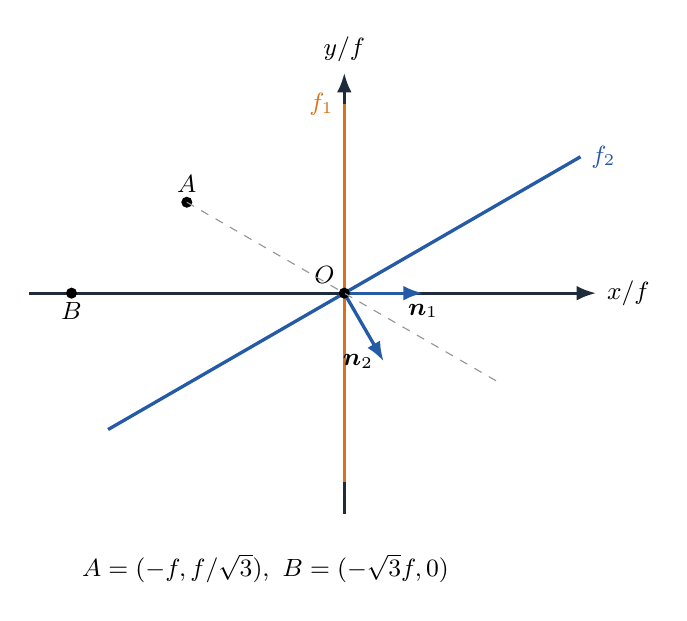
\begin{tikzpicture}[x=1cm,y=1cm,font=\small]

\draw[axis](-4,0)--(3.2,0)node[right]{$x/f$};\draw[axis](0,-2.8)--(0,2.8)node[above]{$y/f$};
\draw[body,orange](0,-2.4)--(0,2.4)node[left]{$f_1$};\draw[body,blue](-3,-1.732)--(3,1.732)node[right]{$f_2$};
\draw[vec](0,0)--(1,0)node[below]{$\boldsymbol n_1$};\draw[vec](0,0)--(.5,-.866)node[left]{$\boldsymbol n_2$};
\fill(-2,1.1547)circle(2pt)node[above]{$A$};\fill(-3.464,0)circle(2pt)node[below]{$B$};\fill(0,0)circle(2pt)node[above left]{$O$};
\draw[guide](-2,1.1547)--(2,-1.1547);\node at(-1,-3.5){$A=(-f,f/\sqrt3),\ B=(-\sqrt3f,0)$};
\end{tikzpicture}

% 14 solution-07
\begin{tikzpicture}[x=1cm,y=1cm,font=\small]

\draw[axis](-4,0)--(3.2,0)node[right]{$x/f$};\draw[axis](0,-2.8)--(0,2.8)node[above]{$y/f$};
\draw[body,orange](0,-2.4)--(0,2.4)node[left]{$f_1$};\draw[body,blue](-3,-1.732)--(3,1.732)node[right]{$f_2$};
\draw[vec](0,0)--(1,0)node[below]{$\boldsymbol n_1$};\draw[vec](0,0)--(.5,-.866)node[left]{$\boldsymbol n_2$};
\fill(-2,1.1547)circle(2pt)node[above]{$A$};\fill(-3.464,0)circle(2pt)node[below]{$B$};\fill(0,0)circle(2pt)node[above left]{$O$};
\draw[guide](-2,1.1547)--(2,-1.1547);\fill (2.000000,-1.154700) circle(2pt) node[below] {$A_{12}'=A_{21}'$};
\fill (2.167670,0.000000) circle(2pt) node[above] {$B_{12}'=B_{21}'$};
\node[align=left,anchor=west]at(4,0){A首次为无穷远像\\终像 $(f,-f/\sqrt3)$\\B终像 $(1.083835f,0)$\\法向点积使用带符号坐标};
\end{tikzpicture}

% 15 question-08
\begin{tikzpicture}[x=1cm,y=1cm]
  \coordinate (A) at (-4,-2.3); \coordinate (B) at (4,-2.3); \coordinate (C) at (0,4.63);
  \draw[body] (A)--(B)--(C)--cycle;
  \coordinate (P) at ($(A)!2/3!(B)$); \coordinate (Q) at ($(B)!2/3!(C)$); \coordinate (R) at ($(C)!2/3!(A)$);
  \draw[very thick,blue] (P)--(Q)--(R)--cycle;
  \coordinate (P2) at ($(P)!2/3!(Q)$); \coordinate (Q2) at ($(Q)!2/3!(R)$); \coordinate (R2) at ($(R)!2/3!(P)$);
  \draw[very thick,orange] (P2)--(Q2)--(R2)--cycle;
  \node[below left] at (A) {$A$}; \node[below right] at (B) {$B$}; \node[above] at (C) {$C$};
  \draw[dim] (-4.65,-2.3)--(-.65,4.63) node[midway,left] {$l$};
  \node[align=center] at (0,-3.15) {每一级在上一级三边的循环三等分点处内接正三角形};
\end{tikzpicture}

% 16 solution-08
\begin{tikzpicture}[x=1cm,y=1cm]
  \coordinate (A) at (-4,-2.3); \coordinate (B) at (4,-2.3); \coordinate (C) at (0,4.63);
  \coordinate (P) at ($(A)!2/3!(B)$); \coordinate (Q) at ($(B)!2/3!(C)$); \coordinate (R) at ($(C)!2/3!(A)$);
  \draw[body] (A)--(P)--(B)--(Q)--(C)--(R)--cycle;
  \draw[very thick,blue] (P)--(Q)--(R)--cycle;
  \foreach \p/\t/\pos in {A/A/below left,B/B/below right,C/C/above,P/P/below,Q/Q/right,R/R/left}{\node[nodept] at (\p) {};\node[\pos] at (\p) {$\t$};}
  \node[below] at ($(A)!.5!(P)$) {$2rl/3$}; \node[below] at ($(P)!.5!(B)$) {$rl/3$};
  \node[blue,right] at ($(P)!.5!(Q)$) {$x$};
  \node[align=left,anchor=west] at (4.6,2.5)
    {$X_n=\dfrac{3x+2rl}{3(x+rl)}\,rl$\\[3pt]
     $x=\dfrac1{\sqrt3}X_{n-1}$\\[3pt]
     $R_n=\dfrac23X_n$};
  \node[align=center] at (0,-3.15) {内层三端网络因三重旋转对称，可等效为三条相同电阻组成的三角形};
\end{tikzpicture}
\end{document}
